\chapter{Code Validation}\label{appendix:code_test}
In order to check the reliability of the implemented LOCO code and also to develop an intuition on the method behavior for the Sirius storage ring (before actual applications), a series of tests were performed. In this appendix these tests and the results obtained are reported.

\section{Detecting Distributed Errors}
The first test to check the implemented code consists in perturbing the simulated storage ring model, obtain the corresponding~\gls{orm} and then trying to determine the input errors from the fit parameters with LOCO analysis. 
% In this way, since the planted errors perturbs the~\gls{orm} and~\gls{loco} tries to adjust the fit parameters until the goal~\gls{orm} is fitted, once the perturbed~\gls{orm} is explained by~\gls{loco}, the corresponding changes in the fit parameters should match the input errors. 

% This test simulates the usage of~\gls{loco} as a diagnostic tool. However, since the only errors in the simulated model was included in the elements that was already adjusted in~\gls{loco}, subtracting the negative fit values in the perturbed model cancels out the input errors and in this way~\gls{loco} also can be viewed as a correction tool.

It is important to point out that this test should work properly if the errors are included in the elements that are used as fit parameters in LOCO method. For example, if gradient errors are added in the sextupoles but only quadrupoles strengths are fitted, the quadrupoles will be changed to best fit the~\gls{orm}. Thus, even if the $\chi^2$ is reduced, the final quadrupoles variations will not match the planted gradient errors in the sextupoles, since these elements are in different positions around the ring, with different phase advances. In this case, the fitted values must be interpreted only as the gradient changes in quadrupoles that best explain the perturbed \gls{orm}. Clearly this type of compensation should reach a limit of fitting effectiveness. Therefore, whenever it is possible, the most appropriated approach is to identify and then to minimize the errors sources not covered by LOCO and, only after that, apply~\gls{loco} analysis to obtain appropriated corrections.

A hundred sets of errors were generated following a random normal distribution with $3\sigma$ cutoff. These errors were included in the simulated model and then the corresponding hundred~\gls{orm}s were calculated. LOCO analysis were performed for these~\gls{orm}s, fitting all the parameters described in Table~\ref{tab:fit_params}. The~\gls{std} $\sigma$ used in the normal distribution to generate random errors for each parameter are presented in Table~\ref{tab:errors}.
\begin{table}[h!]
    \centering
    \caption{Random errors included in the simulated model ($3\sigma$ cutoff).}
    \label{tab:errors}
    \begin{tabular}{ccc}
        \toprule\toprule
        Parameter & $\sigma$ of distribution & Unit\\ 
        \hline
        Normal quadrupole gradient & 0.1 &\% \\
        H. and V. BPM gain &  2.5 & \% \\
        H. and V. Corrector gain & 5.0 &\% \\
        Skew quadrupole gradient & $10^{-3}$ &$\SI{}{\meter^{-1}}$ \\
        % V. BPM gain &  10 & \% \\
        BPM roll angle & 10 & $\SI{}{\milli\radian}$ \\ 
        % V. Corrector gain &  10 &\% \\
        \bottomrule\bottomrule
    \end{tabular}
\end{table}

The goal of this test is to compare the fitted variations determined from~\gls{loco} with the random errors included in the model. The statistics related to the differences between these two sets of values are presented in Table~\ref{tab:diff_target}, where the difference was normalized by the~\gls{std} $\sigma$ used to generate the random errors.
% \begin{table}
%     \centering
%     \caption{Differences (normalized by $\sigma$) between planted errors and fitted variations obtained from LOCO analysis for 100 sets of random errors.}
%     \label{tab:diff_target}
%     \begin{tabular}{ccc}
%         \toprule\toprule
%         Parameter & mean difference$/\sigma$ & peak-to-valley difference$/\sigma$  \\ 
%         \hline
%         Normal quadrupole gradient & \num{9.8e-3}& $\SI{3.4e-2}{}$\\
%         H. BPM gain & $\SI{1.9e-4}{}$  & $\SI{7.9e-4}{}$\\
%         H. Corrector gain & $\SI{7.5e-5}{}$ &  $\SI{2.7e-4}{}$ \\
%         V. BPM gain & $\SI{7.7e-4}{}$ & $\SI{1.7e-3}{}$\\
%         V. Corrector gain & $\SI{7.7e-4}{}$ & $\SI{1.7e-3}{}$ \\
%         Skew quadrupole gradient & $\SI{3.9e-3}{}$  & $\SI{1.4e-2}{}$ \\
%         BPM roll angle & $\SI{3.8e-3}{}$ & $\SI{1.3e-2}{}$ \\
%         \bottomrule\bottomrule
%     \end{tabular}
% \end{table}
\begin{table}[h!]
    \centering
    \caption{Differences (normalized by $\sigma$) between planted errors and fitted variations obtained from LOCO analysis for 100 sets of random errors.}
    \label{tab:diff_target}
    \begin{tabular}{ccc}
        \toprule\toprule
        Parameter & std difference$/\sigma$ & peak-to-valley difference$/\sigma$  \\ 
        \hline
        Normal quadrupole gradient & \num{1.1e-2}& \num{5.9e-2}\\
        H. BPM gain & \num{2.8e-4} & \num{1.6e-3} \\
        H. Corrector gain & \num{1.0e-4}  & \num{5.5e-4}  \\
        V. BPM gain & \num{7.8e-4} & \num{3.2e-3} \\
        V. Corrector gain & \num{7.9e-4} & \num{3.2e-3} \\
        Skew quadrupole gradient & \num{4.9e-3} & \num{2.3e-2} \\
        BPM roll angle & \num{4.7e-3} & \num{2.2e-2} \\
        \bottomrule\bottomrule
    \end{tabular}
\end{table}

From the results in Table~\ref{tab:diff_target} it can be seen that for the normal quadrupoles, skew quadrupoles and BPM roll angles, target and obtained errors normalized by $\sigma$ agrees to within a few percent. For the gains of horizontal correctors and BPM, the difference is a few parts in ten thousand and for the vertical ones, it is a few parts in a thousand. The dispersion function was included in the fitting to break the horizontal gains degeneracy, which explains the fact that the gains determination for the horizontal plane was more efficient than the obtained in the vertical plane.
\begin{figure}
\centering
\begin{subfigure}[t]{0.49\textwidth}
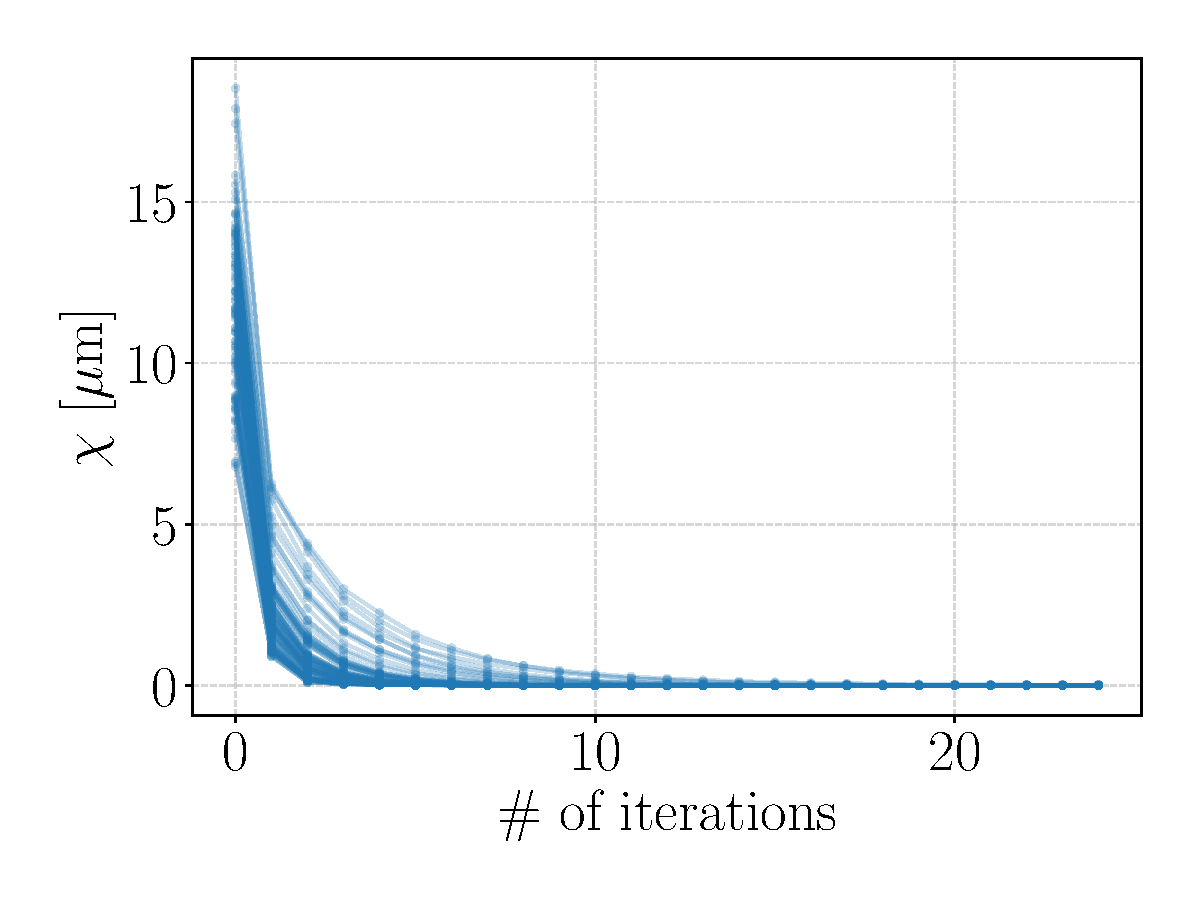
\includegraphics[width=1.0\textwidth]{figures/chi_seeds_grid_big.pdf}
    \caption{$\chi$ convergence.}
    \label{subfig:chi_seeds}
\end{subfigure}
 \begin{subfigure}[t]{0.49\textwidth}
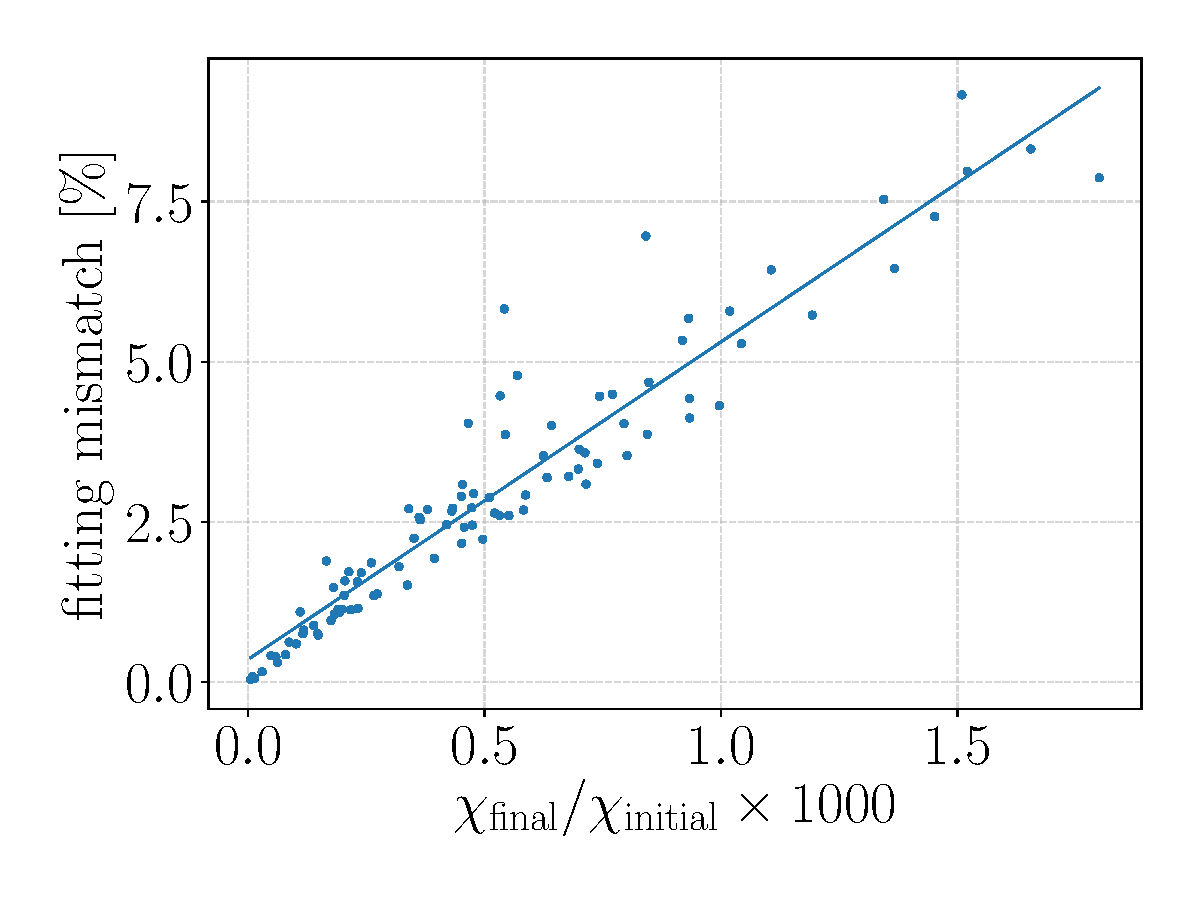
\includegraphics[width=1.0\textwidth]{figures/chi_versus_score_grid_big.pdf}
    \caption{Fitting mismatch versus fitting level.}
    \label{subfig:chi_versus_score}
\end{subfigure}
\caption{Fitting over 100 random ORM obtained from the simulated model.}
\label{fig:fitting_seeds}
\end{figure}
The average initial $\chi$ for these 100 sets of random errors was $\SI{11.6}{\micro\meter}$ and after the fitting, the average final $\chi$ was $\SI{6.2}{\nano\meter}$. Such level of fitting is only possible because in these tests the~\gls{orm} was obtained without any noise in the data and the process is not subjected to measurement errors. For real measurements, it is desired to achieve a final value for $\chi$ that is close to the BPM accuracy, which with the current technology is typically from hundreds of nanometers to a few micrometers.

In Figure~\ref{subfig:chi_seeds} the convergence of $\chi$ for the 100 fittings is presented. The maximum number of iterations was limited to 25. It can be seen that at about 15 iterations $\chi$ already converged for all the 100 cases. Figure~\ref{subfig:chi_versus_score} shows the relation between the fitting level, represented by the ratio $\chi_{\mathrm{final}}/\chi_{\mathrm{initial}}$, and the fitting mismatch for each realization, obtained by $\sqrt{\sum_{p}d_p^2}$, where $d_p$ is the difference between target and fitted errors normalized by $\sigma$ for the parameter $p$ covering all the 7 fit parameters used in LOCO runs. The mismatch in the fitting grows linearly with the fitting level, with a proportionality factor of about 50. The code would be unreliable if the fitting level was good but the corresponding mismatch was large. Such cases were not observed in the 100 random realizations.
\section{Detecting Localized Errors}
Detecting single errors is very useful to identify, in a more specific way, malfunctioning elements or a problematic region in the storage ring. A functional diagnostic tool that provides this localized detection can spare a considerable amount of time in the investigation of problems that are degrading the machine performance, thus being a helpful tool for the commissioning stage and regular operation of a synchrotron light source as well, since installation and maintenance intervention occurs several times during the machine lifetime. The goal of the tests reported in the present subsection is to check LOCO ability to identify localized errors on quadrupoles, BPMs and correctors. 

\subsection{Single Gradient}
Suppose that amongst random gradient errors in quadrupoles, there is a single quadrupole with a large deviation from its nominal value. Single quadrupole errors are not naturally expected, since magnetic measurements are performed before the assembly in storage ring to guarantee that mechanical and magnetic properties meet the specifications for all magnets. However, after the magnets assembly some kind of problem in a specific magnet coils or in its power supply may appear and lead to localized errors.

The following error distribution was generated and applied in Sirius storage ring model: gaussian random errors in gradient strengths with std $\sigma=\SI{0.25}{\%}$ and $\SI{2.0}{\%}$ of error in the 215\ts{th} quadrupole. Errors in others parameters were not included. An~\gls{orm} was calculated with this perturbed model and it was used as input for LOCO analysis, including all fit parameters. The results for variations in quadrupoles fitted by LOCO compared to the target errors are in Figure~\ref{fig:single_quad_detec}.
\begin{figure}[h!]
\centering
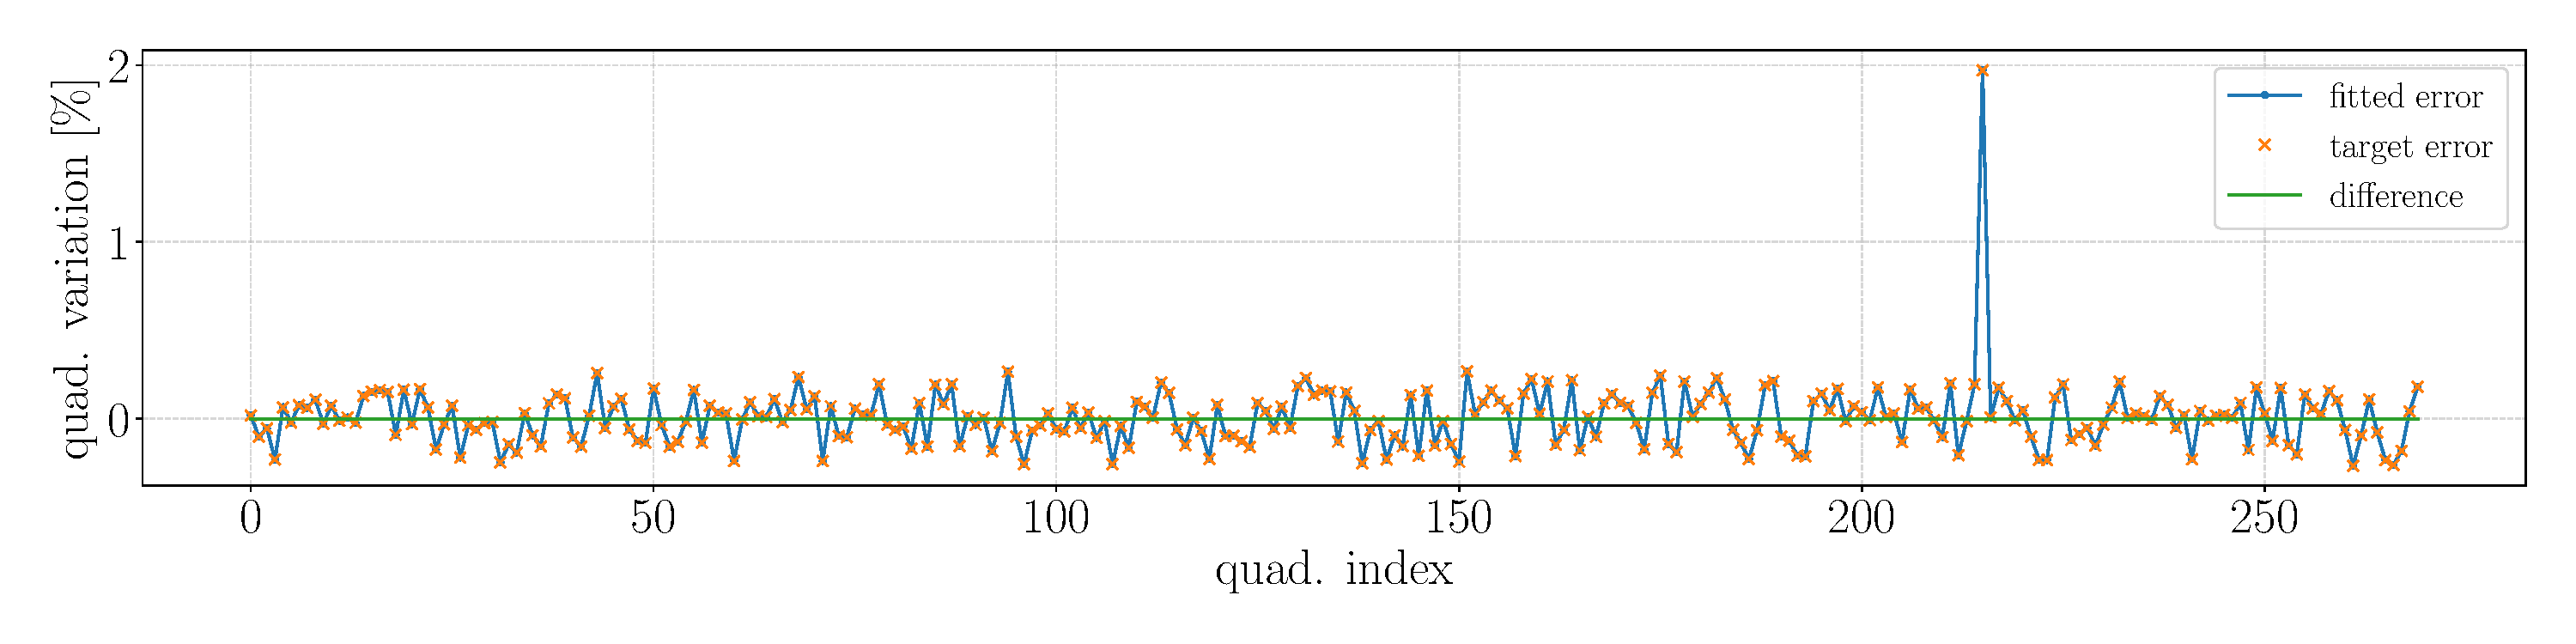
\includegraphics[width=1.0\textwidth]{figures/single_quaderror_detection_big.pdf}
\caption{Fitted and target quadrupoles variations, including a higher error of 2\% in the 215\ts{th} quadrupole.}
\label{fig:single_quad_detec}
\end{figure}

From Figure~\ref{fig:single_quad_detec} it can be seen that the input errors were accurately determined, including the single large gradient error. The maximum difference between fitted and target error for quadrupoles was $\num{1e-8}$. The final value of $\chi$ in this fitting was very low, around $\SI{1e-6}{\micro\meter}$. The variations on the remaining fit were in a much lower level, the maximum variation of BPM gains and correctors was $\num{3e-6}$ and for skew quadrupoles strengths $\SI{1e-16}{\meter^{-1}}$, on the order of computer numeric precision.

It is clear that this level of error determination is only possible for tests in the simulated model, when the goal~\gls{orm} was obtained without noise and measurement errors. Nevertheless, in the limit that these practical limitations are set as low as possible in real measurements, it would still be possible to identify single errors with reasonable accuracy.
\subsection{Single Gain}
The same tests were performed with BPMs and correctors gains. Such type of error in gains may be associated with malfunctioning in~\glspl{bpm} antennas, electrical interference or software issues. For correctors the outliers in gains may indicate problems in the magnet coils or in its power supplies. For BPMs, the problems are typically easier to detect since they can be identified directly from unrealistic position measurements. For correctors, the effect on the beam produced by localized problems may be more subtle to identify directly. Measuring the~\gls{orm} and performing LOCO analysis is usually a good indirect procedure to detect the aforementioned errors.

Gaussian random errors with std $\sigma=\SI{10}{\%}$ were applied both for horizontal and vertical gains. BPM roll angle errors were included following a gaussian random distribution with std $\sigma=\SI{1}{\milli\radian}$.  The corresponding gains for 7\ts{th} BPM, CH and CV were increased by a $1.5$ factor. This means that the nominal~\gls{orm}, after applying the random gains errors, had the 7\ts{th} and 167\ts{th} rows (for the 7\ts{th} BPM) and 7\ts{th} and 127\ts{th} columns (for the 7\ts{th} CH and CV) multiplied by $1.5$. This altered~\gls{orm} were set as the goal matrix for LOCO fitting, where all fit parameters were included again. The fitting results for this test are shown in Figure~\ref{fig:gain_greater}.
\begin{figure}[h!]
\centering
\begin{subfigure}[t]{0.49\textwidth}
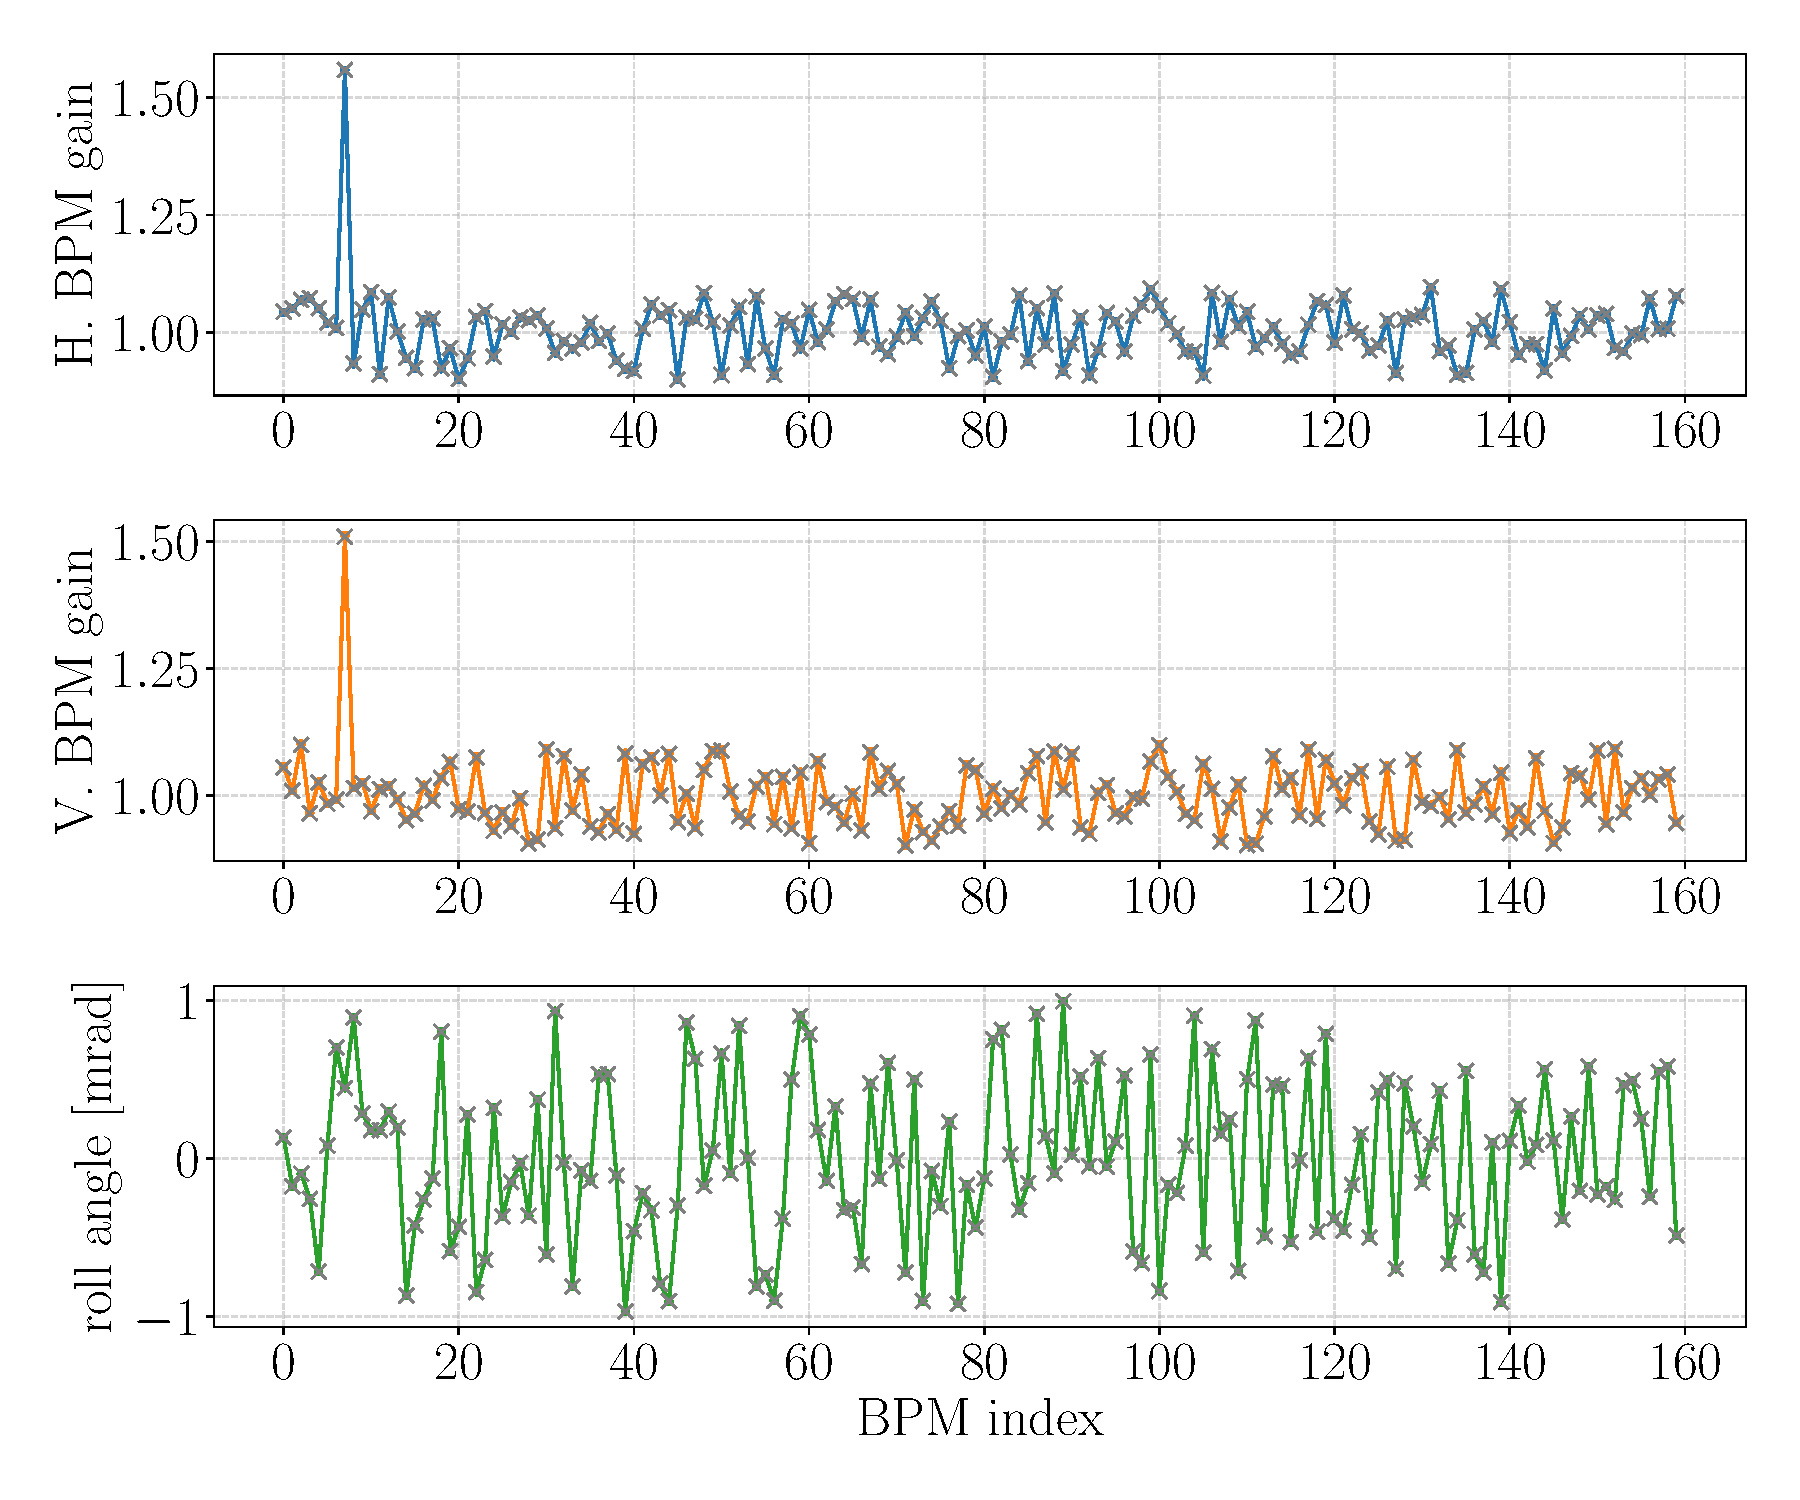
\includegraphics[width=1.0\textwidth]{figures/bpm_gains_1p5gain_7th_bpm_grid_big.pdf}
    \caption{BPM gains and roll angles.}
    \label{subfig:bpm_fit_gain_greater}
\end{subfigure}
 \begin{subfigure}[t]{0.49\textwidth}
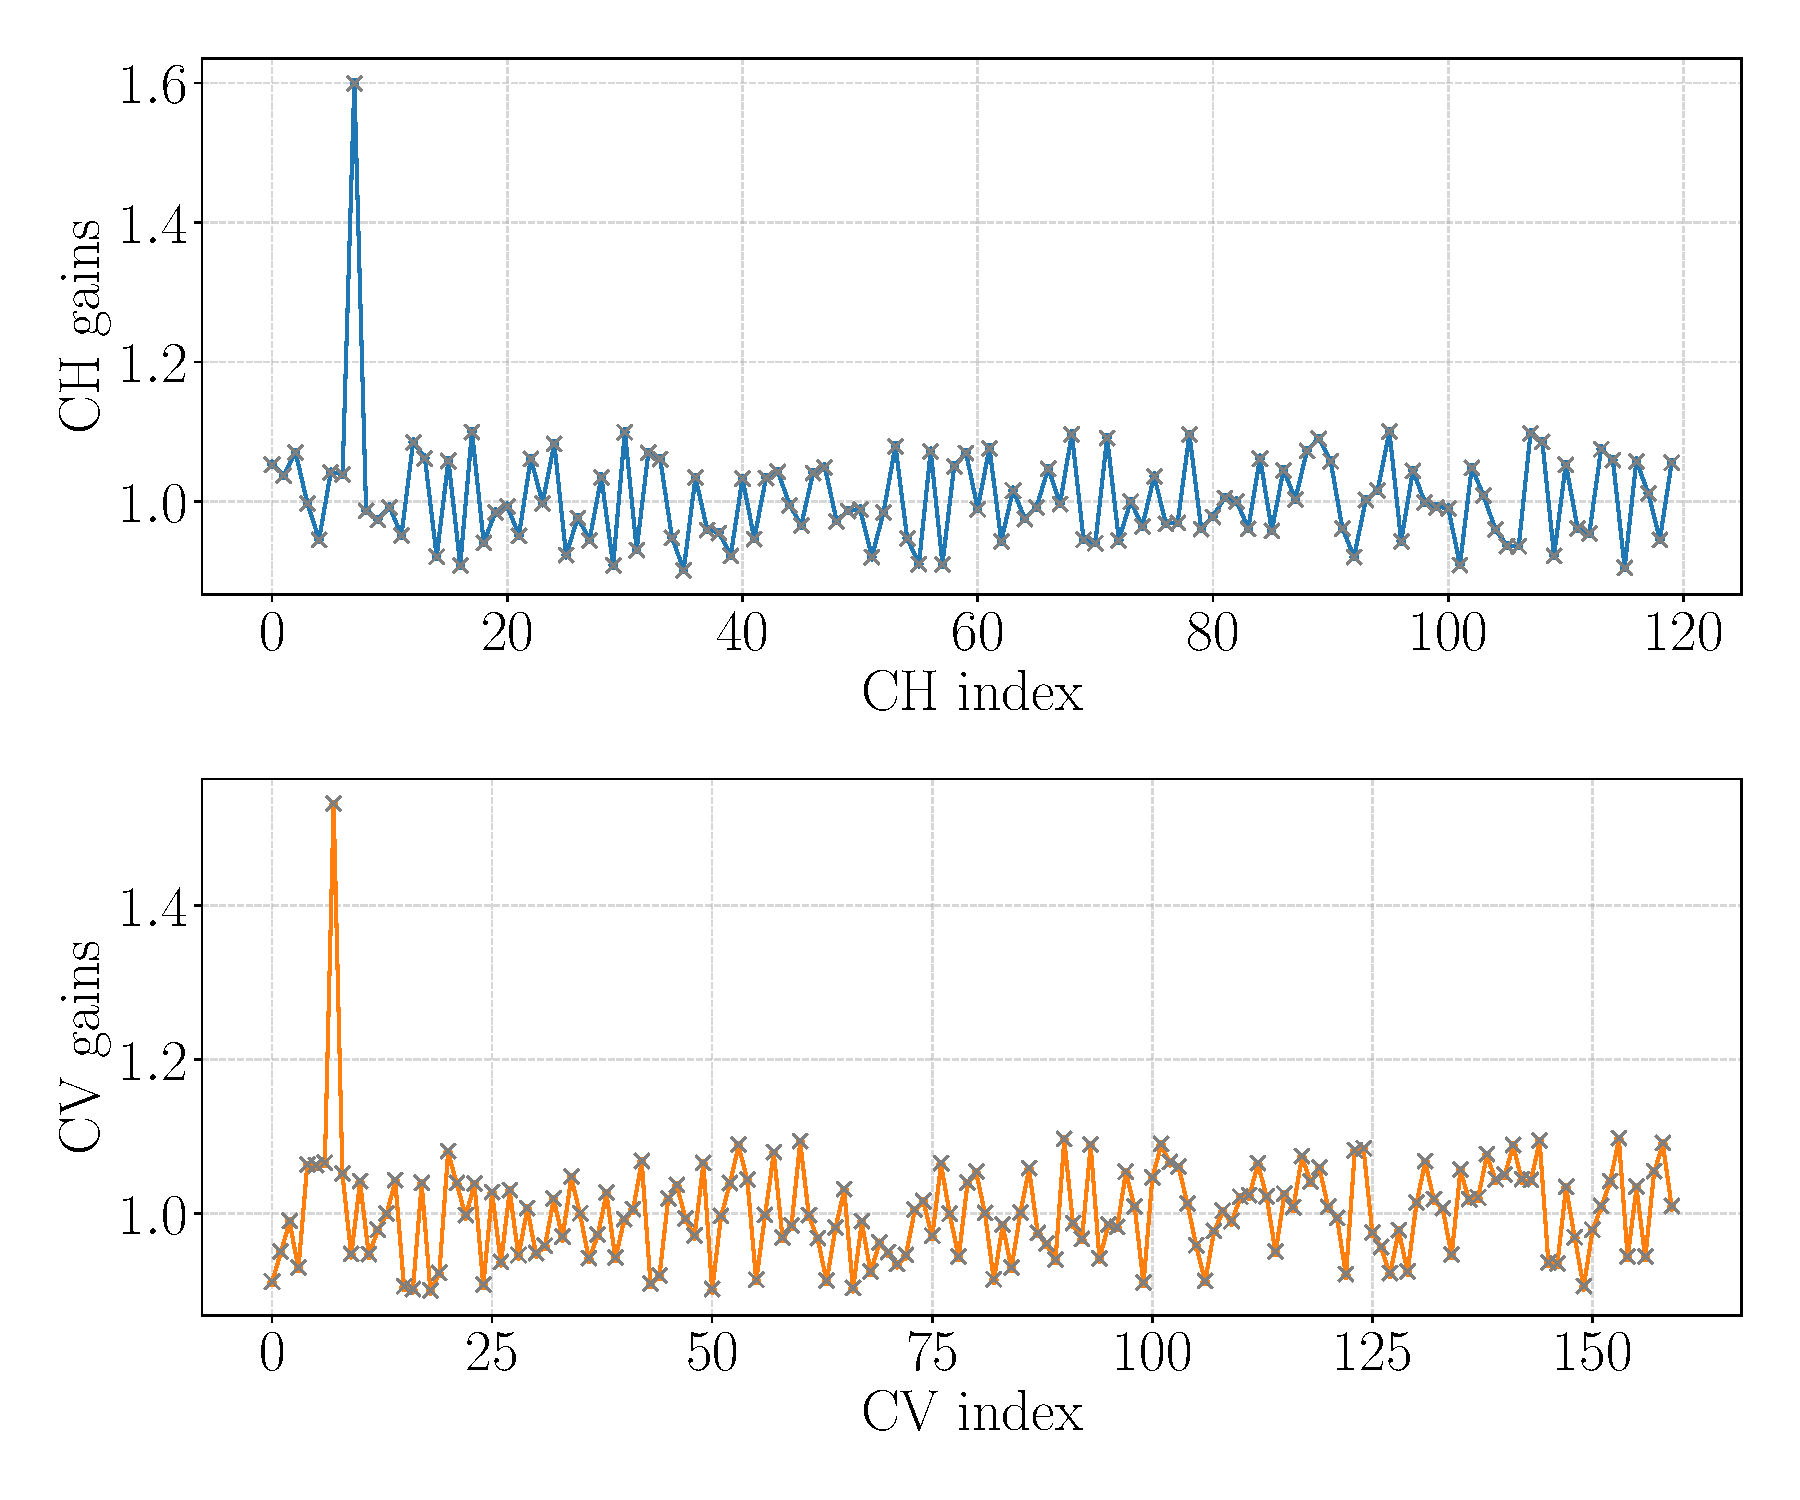
\includegraphics[width=1.0\textwidth]{figures/corr_gains_chcv_1p5_grid_big.pdf}
    \caption{Correctors gains.}
    \label{subfig:corr_fit_gain_greater}
\end{subfigure}
\caption{Fitted values for BPM gains, roll errors and correctors (CH and CV) gains, where the 7\ts{th} BPM, CH and CV gains are greater by a 1.5 factor. Gray $\times$ represents the target errors.}
\label{fig:gain_greater}
\end{figure}

Once again, the input errors were determined precisely and the larger planted gains were identified, both for BPM and correctors. The maximum difference between fitted and target error for horizontal gains (BPM and CH) was $\SI{0.2}{\%}$ and for vertical gains (BPM and CV) was $\SI{0.1}{\%}$. The other parameters were changed again in a lower level, the maximum variation for quadrupoles was $\SI{2e-6}{}$ and for skew quadrupoles $\SI{4e-9}{\meter^{-1}}$.